\chapter{Background}\label{chap:background}

The following will provide an introduction into some of the core concepts necessary to understand how Polish cryptologists were able to break Enigma in 1932. We will introduce the hardware of the Enigma machine, as well as provide a brief overview of permutation theory. We will also prove a theorem which is integral in creating the permutations used in the set of equations that model the electrical circuit inside Enigma.

\section{Enigma Hardware}

\begin{figure}[h!]
\begin{centering}
  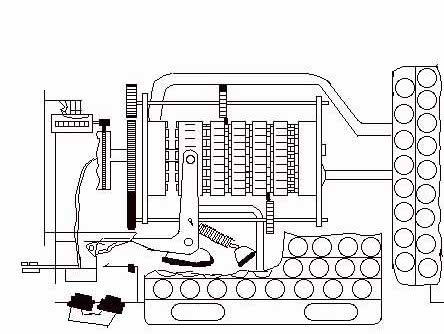
\includegraphics[height=10cm]{images/rotors.jpg}
  \caption{Hardware of the Enigma Machine}
  \label{fig:hardware1}
\end{centering}
\end{figure}

In order to understand how the ciphertexts created by the Enigma machine were broken, it is important to understand the inner workings of the machine itself. Figure \ref{fig:hardware1} shows a schematic of the hardware.

On the outside of each machine, there is a keyboard and a row of glowlamps. Each key on the keyboard is connected to a glowlamp through a changing electric circuit, so when a key is pressed it lights up a corresponding glowlamp. Below the keyboard, there is a plugboard with between six (6) and twelve (12) switches. These switches allow for two letters of the alphabet to be transposed prior to being sent into the machine's hardware. It introduced a "reciprocal monoalphabetic substitution between the keyboard and the first rotor" \cite{bw05}. This adds a layer of security beyond the rotors on the inside of the machine.

Inside each machine, there are anywhere from three (3) to as many as eight (8) rotors and a reflector (or reversing drum). These rotors are the main ciphering components. Each rotor has the alphabet inscribed on the rim, twenty-six (26) fixed contacts on one face, and twenty-six (26) spring loaded contacts on the other face \cite{wk85}. Each rotor has a unique circumference, as well as a unique set of connected contacts. These contacts are randomly connected, and are different on each rotor \cite{bw05}. The reversing drum is responsible for creating the reciprocal nature of the machine, meaning that if an 'A' is pressed on the keyboard and an 'F' lights up on the glow lamps, it also means that if an 'F' is pressed on the keyboard, the 'A' will light up on the glow lamps.

Each rotor inside the machine is set up in such a way that it will rotate corresponding to different key presses. The rotor closest to the keyboard rotates every time a key is pressed, meaning that the substitution changes every time a key is pressed. The other two (2) to seven (7) rotors rotate at variable rates, depending on how the hardware is configured. The second rotor's rotation is dependent on the first rotor's rotation, the third rotor is dependent on the second, and so on and so forth. This rotation of the rotors adds another level of complexity on top of the already complex substitution cipher that Enigma creates.

\section{Important Mathematical Concepts}\label{sec:mathconcepts}

To understand some of the mathematical theory later on in this paper, one must first understand some basics of permutation groups. A permutation is a rearrangement of elements in a set. An example of this kind of permutation is rearranging the numbers ${1,2,3,4,5}$ into ${3,5,4,2,1}$. This could be expressed in the standard matrix form
$P = \begin{pmatrix}
    1 & 2 & 3 & 4 & 5 \\
    3 & 5 & 4 & 2 & 1
  \end{pmatrix}$, or in cyclic notation as $P_c = (1 3 4 2 5)$. Notice in cyclic notation that there is an implied transposition from $5$ to $1$ from the last element in $P_c$.

Permutations can be multiplied as well. In multiplying permutations, order is important. If we have
$$P = \begin{pmatrix}
    1 & 2 & 3 & 4 & 5 \\
    3 & 5 & 4 & 2 & 1
  \end{pmatrix}$$

$$Q = \begin{pmatrix}
    1 & 2 & 3 & 4 & 5 \\
    2 & 1 & 4 & 3 & 5
  \end{pmatrix}$$

One can multiply

$$QP = \begin{pmatrix}
    1 & 2 & 3 & 4 & 5 \\
    2 & 1 & 4 & 3 & 5
  \end{pmatrix}
  \begin{pmatrix}
    1 & 2 & 3 & 4 & 5 \\
    3 & 5 & 4 & 2 & 1
  \end{pmatrix}$$

To multiply, rearrange the columns of the $Q$ permutation (leftmost) so that the first row matches the $P$ permutation (or the rightmost). Then, take the non-matching rows of $P$ and $Q$ as the product. In this example, we get

$$QP = \begin{pmatrix}
    1 & 2 & 3 & 4 & 5 \\
    2 & 1 & 4 & 3 & 5
  \end{pmatrix}
  \begin{pmatrix}
    1 & 2 & 3 & 4 & 5 \\
    3 & 5 & 4 & 2 & 1
  \end{pmatrix} =
  \begin{pmatrix}
    3 & 5 & 4 & 2 & 1 \\
    4 & 5 & 3 & 1 & 2
  \end{pmatrix}
  \begin{pmatrix}
    1 & 2 & 3 & 4 & 5 \\
    3 & 5 & 4 & 2 & 1
  \end{pmatrix} =
  \begin{pmatrix}
    1 & 2 & 3 & 4 & 5 \\
    4 & 5 & 3 & 1 & 2
  \end{pmatrix}
  $$

In cyclic notation, $QP = (1 4)(2 5)(3)$.
\\

Another important concept necessary in order to fully understand the theory behind cracking the Enigma machine cipher is the \textit{Theorem on the Product of Transpositions}. First, a transposition is a 2-cycle permutation, for example $P = (13)$. A group of disjunctive transpositions, then, is a group of non-overlapping 2-cycles.
\\

The Theorem on the Product of Transpositions states that:
\\

\textit{If two permutations of the same degree consist solely of disjunctive transpositions, then their product will include disjunctive cycles of the same lengths in even numbers.}
\\

The proof is as follows:
\\

We assign two permutations to be multiplied to be $X$ and $Y$, with total degree $2n$. If both $X$ and $Y$ have identical transpositions within them, such as $(ab)$, then the product will have two distinct cycles $(a)$ and $(b)$. This makes up our base case, as any two permutations with identical transpositions will have an even number of disjunctive transpositions.

Our next step occurs as such. If permutation $X$ includes a transposition $(a_1 a_2)$, there must be a permutation in $Y$ that begins with $a_2$, such as $(a_2 a_3)$. We have already ruled out the possibility of $Y$ including $(a_2 a_1)$ in our base case. We can continue this logic and say the following:

$$(a_1 a_2), (a_3 a_4), ..., (a_{2k-3} a_{2k-2}), (a_{2k-1} a_{2k}) \in X$$
$$(a_2 a_3), (a_4 a_5), ..., (a_{2k-2} a_{2k-1}), (a_{2k} a_{1}) \in Y$$

From these two sets $X$ and $Y$, when we multiply them together we will always obtain two cycles of the same length $k \leq n$:

$$(a_1 a_3 ... a_{2k-3} a_{2k-1}) (a_{2k} a_{2k-2} ... a_4 a_2)$$

We continue this step until there are no more elements in $X$ and $Y$, with the result that the product will only include disjunctive cycles of the same lengths in even numbers, which concludes the proof. This proof was adapted from Appendix E from Kozaczuk \cite{wk85}.

In the breaking of Enigma, Polish mathematicians also used the converse of the above proof, which states that \textit{if a permutation of even-numbered degree includes disjunctive cycles of the same lengths in even numbers, then this permutation may be regarded as a product of two permutations, each consisting solely of disjunctive transpositions}.
